\chapter{各种应用}
介绍Linux下面常用的各类程序。本章用到且OBS中没有的软件源一般写在\ref{repo}中。
\section{影音播放}
\emp{首先请安装好\href{https://lug.ustc.edu.cn/sites/opensuse-guide/codecs.php}{解码器},否则某些格式将无法播放!}安装解码器等的时候,可能会遇到依赖关系导致的冲突的问题。
冲突的解决请参见\href{https://forum.suse.org.cn/viewtopic.php?t=2867&p=22491#p22491}{安装软件碰到冲突,应该如何选择解决方式?}执行完这一步你的Packman源
就应该添加好了,如果你认为这个源太慢,请尝
试Packman的\href{http://packman.links2linux.org/mirrors}{镜%
像源}
\begin{compactdesc}
 \item[电影] \soft{smplayer},或者\soft{vlc}。
 \item[音乐] 默认的\soft{amarok}与KDE环境集成较好。或者\soft{deepin-music},它启用\href{https://forum.suse.org.cn/viewtopic.php?f=7&t=2530}{百度插件}后便能够下载歌曲了。
\end{compactdesc}

\section{文档处理}
\paragraph{\TeX}推荐Kile作为前端,这种情况下你只需要
\begin{Verbatim}[formatcom=\color{codec}]
    sudo zypper in kile texlive-ctex texlive-savesym
\end{Verbatim}
更详细的配置过程请参
考\LaTeX 的\href{https://forum.suse.org.cn/viewtopic.php?f=6&t=2392&p=18750}{配置指南}。除此之外你还可
以用\TeX studio, \TeX works,VIM和Emacs等各种编辑器。本文就使用\LaTeX排版。

\paragraph{Office}LibreOffice、永中Office或WPS。安装好WPS后需要下载\href{http://pan.baidu.com/s/1ntMEU2P}{Symbols}字体并安装之。否则无法显示各种数学符号等。另外由于WPS是32位的程序,所以如果你是64位操作系统请额外安装\soft{cups-libs-32bit},否则WPS无法输出文档为pdf。
\section{教育程序}
\paragraph{词典} 推荐\soft{goldendict}\footnote{请务必安装版本号大于1.5的版本或dev版本,否则无法读取.mdx格式},词典请上\href{http://pdawiki.com/forum/forum.php}{pdawiki}下载,
为了让你的词典更聪明,请下载\href{https://zpj.blog.ustc.edu.cn/wp-content/uploads/2014/02/wordsrule.tar.gz}{构词法}。除此之外还有Stardict,命令行下有sdcv。

\begin{figure}[htbp!]
\centering
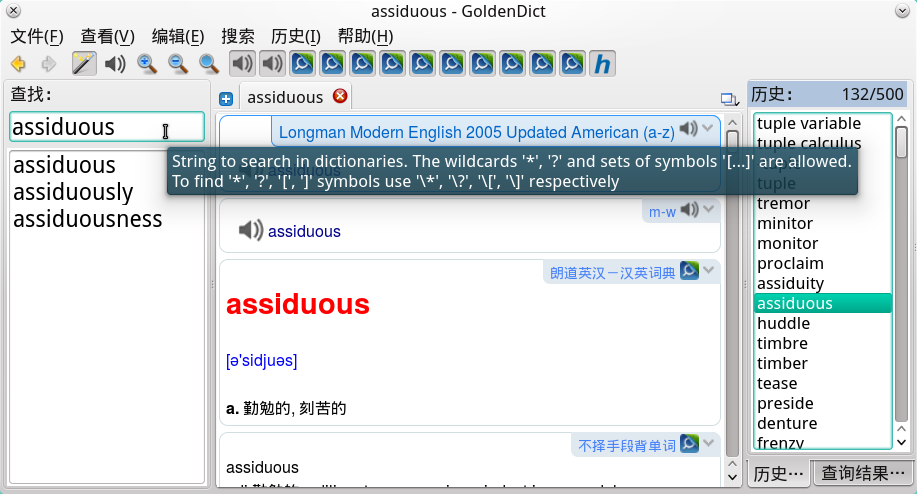
\includegraphics[width=\textwidth]{./pic/goldendict.png} 
\caption{Goldendict}\label{goldendict}
\end{figure}

\paragraph{科学计算、数据处理}\soft{octave}、\textsc{Matlab}、Mathematica、\soft{maxima}、R(\soft{R-base})
\section{图像处理}
\paragraph{点阵图}\soft{gimp}

\begin{figure}[htbp!]
\centering
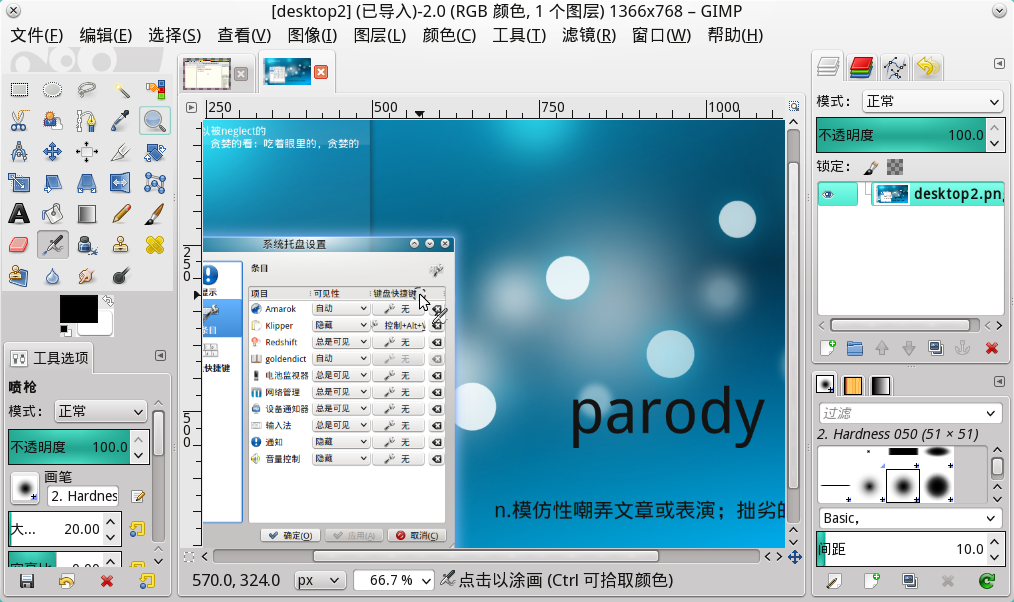
\includegraphics[width=\textwidth]{./pic/gimp.png} 
\caption{Gimp}\label{gimp}
\end{figure}

\paragraph{矢量图}\soft{inkscape}
\section{浏览器}
openSUSE下面默认装有Firefox浏览器,它可以通过安装附加组件来增强其功能。

\paragraph{Firefox}默认安装

\paragraph{Chrome}添加Chrome的源后再搜索\soft{chrome}后安装相应的包即可。

\paragraph{Chromium}添加Packman源后再:
\begin{Verbatim}[formatcom=\color{codec}]
    sudo zypper in chromium chromium-ffmpeg chromium-pepper-flash
\end{Verbatim}
即可安装好Chromium
\section{下载工具}
\begin{compactdesc}
 \item[普通下载] KGet, Firefox的Down\-them\-all!插件,或者直接使用浏览器
 \item[BT] KTorrent, Deluge, Transmition
 \item[ed2k] aMule
\end{compactdesc}

大部分下载都可以用百度网盘这个神器离线下载好,然后再下载到本地。利用有一份田网友的\href{http://git.oschina.net/youyifentian/dupanlink}{百度网盘助手}脚本可以显示百度网盘文件的直接链接。(不过这个助手有时候可能会失效)
\section{网盘与同步盘}
\begin{compactitem}
 \item 坚果云
 \item 百度云在openSUSE下有非官方的\soft{bcloud}客户端
 \item Dropbox
 \item Wuala
 \item etc.欢迎补充
\end{compactitem}
\section{QQ}
腾讯官方提供的QQ for Linux早就无法使用了。webQQ已经挂了,SmartQQ基本半残,只能发送文字——总之很多方法都已经不行了。
但是Chrome和Chromium目前可以运行某些安卓程序,经过测试手机QQ2011可以成功在上面运行。
具体可以参考\href{http://huodong.ustc.edu.cn/Crx}{apk2crx}。